\documentclass[tikz,border=5pt]{standalone}
\usepackage{pgfplots}\usepgfplotslibrary{groupplots}
\pgfplotsset{compat=1.18}
\definecolor{corba}{HTML}{365FB3}\definecolor{segona}{HTML}{0F766E}\definecolor{punt}{HTML}{B91C1C}
\begin{document}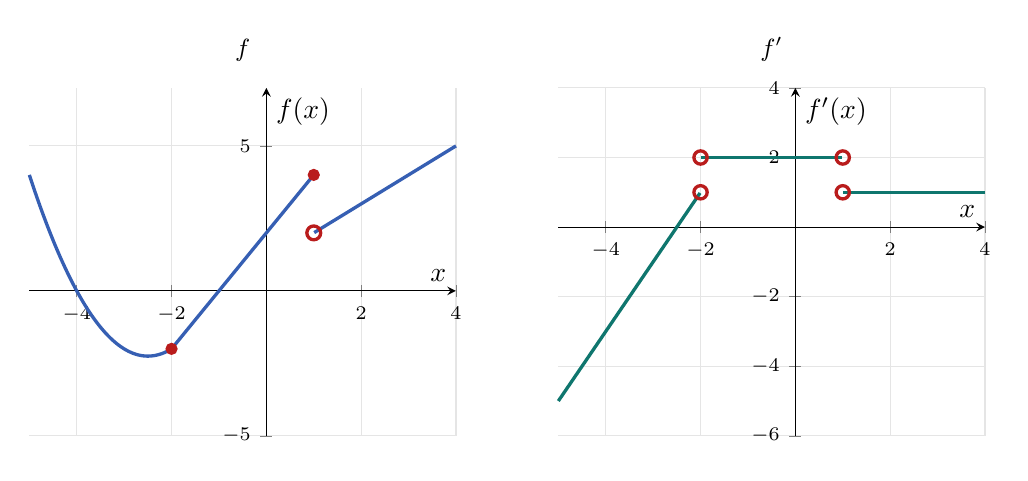
\begin{tikzpicture}
\begin{groupplot}[group style={group size=2 by 1,horizontal sep=1.3cm},width=7cm,height=6cm,
 axis lines=middle,grid=major,grid style={black!10},tick label style={font=\scriptsize},clip=false]
\nextgroupplot[xmin=-5,xmax=4,ymin=-5,ymax=7,xlabel={$x$},ylabel={$f(x)$},title={\small $f$}]
 \addplot[corba,very thick,domain=-5:-2.01,samples=100]{x^2+5*x+4};
 \addplot[corba,very thick,domain=-2:1]{2*x+2};
 \addplot[corba,very thick,domain=1.01:4]{x+1};
 \addplot[only marks,mark=*,mark size=2pt,punt] coordinates {(-2,-2) (1,4)};
 \addplot[only marks,mark=o,mark size=2.5pt,very thick,punt,fill=white] coordinates {(1,2)};
\nextgroupplot[xmin=-5,xmax=4,ymin=-6,ymax=4,xlabel={$x$},ylabel={$f'(x)$},title={\small $f'$}]
 \addplot[segona,very thick,domain=-5:-2.01]{2*x+5};
 \addplot[segona,very thick,domain=-1.99:0.99]{2};
 \addplot[segona,very thick,domain=1.01:4]{1};
 \addplot[only marks,mark=o,mark size=2.4pt,very thick,punt,fill=white] coordinates {(-2,1) (-2,2) (1,2) (1,1)};
\end{groupplot}\end{tikzpicture}\end{document}
